\chapter{مدل‌های مولد مبتنی بر معادلات دیفرانسیل تصادفی}
در دو فصل گذشته دو گونه از مدل‌های پخشی را معرفی کردیم که نقطه‌ی اشتراک هر دو این بود که در یک فرآیند پخش داده را با نویز فزاینده تخریب می‌کردند و سپس در یک فرآیند معکوس از این داده‌ی تخریب شده به مدلی مولد برای تولید داده‌ی جدید می‌رسیدند. در این فصل یک چهارچوب کلی برای فرآیند پخش تعریف می‌کنیم که به جای تخریب داده با یک سری گام گسسته‌ی متناهی، داده را با بی نهایت گام پیوسته تخریب می‌کنیم. این فرآیند تخریب از طریق یک معادله دیفرانسیل تصادفی تعریف شده صورت می‌گیرد و سپس نشان داده می‌شود که برای فرآیند تصادفی یک معادله دیفرانسیل تصادفی معکوس نیز وجود دارد که تنها وابسته به تابع امتیاز می‌باشد. در این بخش ابتدا به معرفی این چهارچوب کلی و مزایای آن می‌پردازیم، سپس ارتباط آن با دو روش پیش‌تر معرفی شده را بیان می‌کنیم و در نهایت به انواع روش‌های نمونه برداری از این توزیع می‌پردازیم.

\section{معرفی فرآیند پخشی با معادلات دیفرانسیل تصادفی}
ایده‌ی اصلی در مدل‌هایی که مبتنی بر معادلات دیفرانسل تصادفی هستند این است که تعداد گام‌های حرکت از توزیع داده به سمت توزیع نویز بی نهایت و به صورت حدی کوچک باشد به طوریکه توزیع داده‌های تخریب شده با افزایش نویز به صورت یک معادله دیفرانسیل تصادفی تغییر کند. مانند مدل‌های قبلی این مدل نیز از سه بخش مسیر رو به جلو، مسیر معکوس و تابع هدف یادگیری تشکیل شده است.تصویر \ref{sde} شمای کلی این روش را نشان می‌دهد.

\begin{figure}[!h]
	\begin{center}
		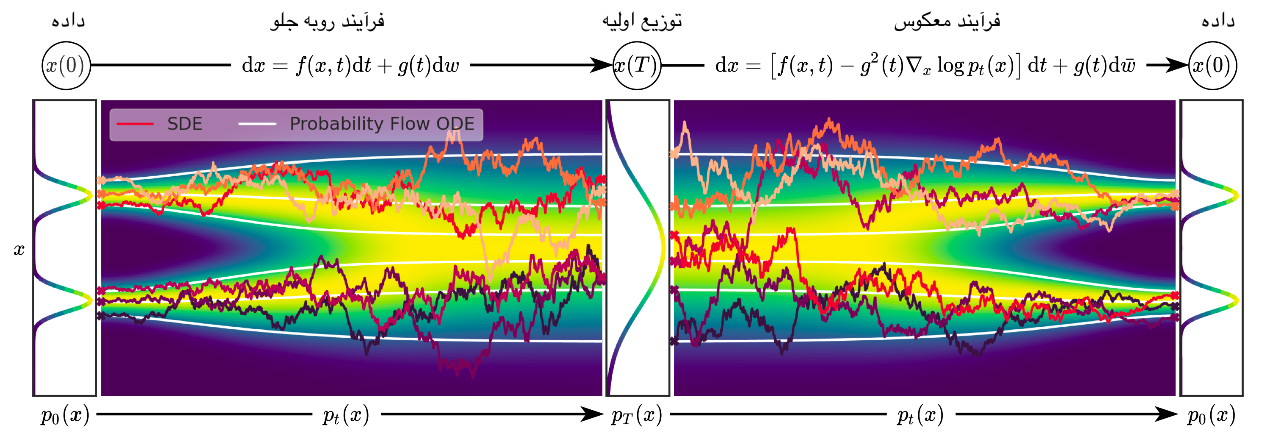
\includegraphics[width=15cm,height=6cm]{sde.png}
		
		\caption{مدل‌های پخشی مبتنی بر معادلات دیفرانسیل}
		\medskip
		\label{sde}
		\small
	مدل‌های پخشی مبتنی بر معادلات دیفرانسیل از فرآیندهای تصادفی و این معادلات برای مدل کردن فرآیند رو به جلو و فرآیند معکوس استفاده می‌کنند\cite{song2020score}.
		
	\end{center}
\end{figure}


\subsection{مسیر روبه جلو}
همانطور که پیش‌تر هم اشاره شد در این مدل هدف توسعه‌ی فرآیند پخش $\left \{ x(t) \right \}_{t=0}^T$ است به طوریکه $x(0) \sim p_0$ یا همان توزیع داده‌ها و $x(T) \sim p_T$ یا همان توزیع اولیه\LTRfootnote{Prior distribution} باشد و متغیر $t$ یک متغیر پیوسته در بازه‌ی $[0,T]$ باشد. در چنین حالتی فرآیند پخش را یک راه حل معادله دیفرانسل تصادفی به فرم زیر در نظر می‌گیریم:

\begin{equation}
	dx = f(x,t)dt + g(t)dw
\end{equation}
که در عبارت بالا $ f(t, .): \mathbb{R}^d \rightarrow \mathbb{R}^d$ ضریب یا تابع رانش\LTRfootnote{Drift coefficient} و $g(.)$ یک مقدار عددی وابسته به زمان است که ضریب پخش\LTRfootnote{Diffusion coefficient} گفته می‌شود. $w$ نیز فرآیند وینر استاندارد\LTRfootnote{Standard wiener process} که معادل همان نویز سفید تصادفی در فضای پیوسته می‌باشد.
به طور کلی توزیع اولیه ی $p_T$ هر توزیع دلخواه قابل محاسبه‌ای است که هیچ اطلاعاتی از توزیع داده در خود ندارد. مانند یک توزیع گاوسی با میانگین و کوواریانس ثابت. حال برای هر توزیع اولیه‌ی مشخص یا هر شکلی از فرآیند پخش یک معادله دیفرانسیل تصادفی طراحی می‌شود که امکان تبدیل توزیع داده به توزیع مشخص شده را دارد.

\subsection{مسیر معکوس}
می‌دانیم که معکوس یک فرآیند پخشی که با معادلات دیفرانسیل مدل می‌شود نیز یک فرآیند پخشی است که در جهت عکس زمانی حرکت می‌کند و با معادله دیفرانسیل تصادفی معکوس زیر مدل می‌شود:
\begin{equation}
	\label{reverse}
	dx = [f(x,t) - g(t)^2\bigtriangledown_x log p_t(x)]dt + g(t)d\bar w
\end{equation}
که $\bar w$ همان فرآیند وینر استاندارد در جهت معکوس از $T$ به $0$ است و $dt$ نیز در جهت منفی حرکت می‌کند\cite{anderson1982reverse}. همانطور که در معادله‌ی(\ref{reverse}) مشاهده می‌شود این عبارت تنها نیازمند تابع امتیاز توزیع $p_t(x)$ می‌باشد و با داشتن این تابع می‌توانیم معکوس فرآیند پخشی را بسازیم و از توزیع داده‌ها نمونه تولید کنیم.

\subsection{تخمین تابع امتیاز}
تابع امتیاز یک توزیع همانطور که در فصل دوم مشاهده شد با فرآیند تطبیق امتیاز قابل تخمین و یادگیری است. تنها نکته‌ی حائز اهمیت این است که در این حالت نیاز به یک تعمیم پیوسته از تابع خطای این شبکه داریم. این تعمیم به صورت زیر قابل بیان است:
\begin{equation}
	\label{cont}
	\theta^\star = \arg\min_{\theta} \mathbb{E}_{t} \left \{ \lambda(t) \mathbb{E}_{x(0)} \mathbb{E}_{(x(t)| x(0))} \left [ \left \| s_\theta(x(t), t) - \bigtriangledown _{x(t)} \log p_{0t}(x(t)| x(0)) \right \|^2_2\right ]   \right \}
\end{equation}

که $\lambda (t)$ یک تابع وزن‌دهی مثبت است و $t$ به صورت یکنواخت از بازه‌ی $[0,T]$ نمونه برداری شده است و $x(0) \sim p_0(x)$ و $x(t) \sim p(x(t)|x(0))$ می‌باشد. اگر ظرفیت مدل مناسب و تعداد داده‌ها کافی باشد معادله ی (\ref{cont}) ما را به پارامترهای بهینه‌ی تابع امتیاز می‌رساند\cite{song2020score}.

\section{مزیت‌های مدل‌های مولد مبتنی بر معادله دیفرانسیل تصادفی}
سه مزیت کلی برای این دسته از روش‌ها می‌توان نام برد که عبارتند از:

\begin{itemize}
	\item
	\textbf{نمونه برداری و محاسبه‌ی درست‌نمایی منعطف: }در این روش از هر حل کننده ی کلی معادلات دیفرانسیل تصادفی برای نمونه گیری از معادله دیفرانسیل تصادفی معکوس می‌توان کمک گرفت. علاوه بر این می‌توان از روش‌های دیگری حل‌کننده های قطعی نیز برای نمونه گیری کمک گرفت.
	\item
	تولید قابل کنترل: از آنجاییکه معادله دیفرانسل تصادفی معکوس شرطی شده از توابع امتیاز غیر شرطی قابل محاسبه است، می‌توانیم فرآیند تولید نمونه را روی اطلاعاتی شرطی کنیم که در حین یادگیری در اختیار مدل قرار نگرفته است. این امر باعث می‌شود تا کاربردهایی مثل ترمیم تصویر\LTRfootnote{Image inpainting}، تولید شرطی شده روی کلاس و رنگ آمیزی\LTRfootnote{Colorization} با یک مدل امتیاز غیرشرطی و بدون آنکه نیاز به آموزش مجدد باشد، قابل انجام باشند.
	\item
	ایجاد یک چهارچوب یکپارچه: این روش قابلیت جستجو و به کارگیری انواع مختلفی از معادلات دیفرانسیل تصادفی را برای بهبود مدل‌های پخشی دارد. همچنین هر دو روش پیش‌تر معرفی شده نیز درقالب این روش قابل بیان و بهینه سازی هستند.
\end{itemize}


\section{ارتباط روش مبتنی بر معادلات دیفرانسیل تصادفی با روش‌های پیش‌تر معرفی شده}
به طور کلی می‌توان گفت فرآیند پخش به کار گرفته شده در مپنا و تطبیق امتیاز با دینامیک لانژوین، گسسته‌سازی‌هایی از روش ارائه شده در این فصل هستند. هر کدام از این روش‌ها از یک معادله دیفرانسیل تصادفی برخوردار هستند که با گسسته‌سازی آن می‌توان هم ارزی روش‌های پیش‌تر معرفی شده را با روش مبتنی بر معادله دیفرانسیل تصادفی نشان داد.
در روش تطبیق امتیازبا دینامیک لانژوین با استفاده از $N$ سطح نویز می‌توان تابع تخریب $p_{\sigma_i}(x|x_0)$ را با توزیع $x_i$ حاصل از یک زنجیره‌ی مارکف به شکل زیر به دست آورد:
\begin{equation}
	x_i = x_{i-1} + \sqrt{\sigma_{i}^2 - \sigma_{i-1}^2} z_{i-1}, \quad i = 1, \ldots, N
\end{equation}

که $z_{i-1} \sim \mathcal{N}(0, I)$ و در صورتی که $N \to \infty$ آنگاه زنجیره‌ی مارکفی بالا به یک فرآیند تصادفی پیوسته به صورت $\left \{ x(t) \right \}_{t-0}^1$ تبدیل می‌شود که خود $t$ هم یک متغیر پیوسته در بازه‌ی $[0,T]$ است. در چنین صورتی می‌توانیم این فرآیند تصادفی را با یک معادله دیفرانسیل تصادفی به فرم زیر مدل کنیم:
\begin{equation}
	\label{VE}
	dx = \sqrt{\frac{d[\sigma^2{(t)}]}{dt}} dw
\end{equation}
این معادله ،که به آن معادله ی انفجار واریانس\LTRfootnote{Variance exploding} می‌گوییم، در واقع حالت خاصی از چهارچوب مطرح شده در این فصل می‌باشد.

به طور مشابه برای مپنا نیز یک زنجیره‌ی مارکفی به شکل زیر داریم:

\begin{equation}
	x_i = \sqrt{1 - \beta_i}x_{i-1} + \sqrt{\beta_i}z_{i-1}, \quad i = 1, \ldots, N
\end{equation}
که در صورتی که $N \to \infty$، به معادله دیفرانسیل تصادفی زیر همگرا می‌شود:
\begin{equation}
	\label{VP}
	dx = -\frac{1}{2}\beta(t)xdt + \sqrt{\beta(t)}}dw
	\end{equation}
	و بنابراین تخریب های نویز به کار برده شده در مپنا و در تطبیق امتیاز با دینامیک لانژوین هر دو گسسته سازی هایی از یک معادله دیفرانسل تصادفی هستند.
	
\section{انواع روش‌های نمونه برداری}
	بعد از آموزش یک شبکه‌ی امتیاز وابسته به زمان می‌توان از آن برای ساخت یک معادله دیفرانسیل تصادفی معکوس استفاده کرد و سپس با استفاده از روش‌های عددی حل این معادله دیفرانسیل آن را شبیه‌سازی و نمونه‌هایی از توزیع $p_0$ تولید کرد. در این قسمت به دو دسته روش حل این معادلات اشاره خواهیم کرد:
\subsection{حل کننده‌های عام منظوره ی معادلات دیفرانسیل تصادفی}
	حل کننده‌های عددی مسیر تقریبی معادلات دیفرانسیل تصادفی را تخمین می‌زنند. بسیاری از این حل کننده‌های عام منظوره مانند روش اویلر-ماریاما\LTRfootnote{Euler-maruyama} برای تولید نمونه به کار گرفته می‌شوند.
	
\subsection{تبدیل به معادلات دیفرانسیل ساده}
	با دانستن تابع امتیاز یک راه دیگر برای حل معادلات دیفرانسیل تصادفی و نمونه برداری، تبدیل این معادلات به معادلات دیفرانسیل ساده\LTRfootnote{Ordinary differential equations} و تبدیل فرآیند تصادفی به فرآیند قطعی\LTRfootnote{Deterministic process} می‌باشد. به ازای هر فرآیند پخشی تصادفی یک فرآیند قطعی متناظر آن وجود دارد که هر دو مسیر توزیع‌های حاشیه‌ای یکسانی دارند. این فرآیند قطعی به صورت زیر قابل بیان است:
	
\begin{equation}
dx = [f(x,t) - \frac{1}{2}g^2(t)\bigtriangledown_x \log p_t(x)]dt
\end{equation}

در صورتی که تابع امتیاز را بدانیم این مسیر به راحتی از معادله دیفرانسیل تصادفی قابل محاسبه است. استفاده از معادلات دیفرانسیل ساده به جای معادلات دیفرانسیل تصادفی مزیت های متعددی از جمله توانایی محاسبه‌ی دقیق درست‌نمایی، کدگذاری یکتا و نمونه برداری کارا دارد.

